\chapter{Les outils informatiques existants}
\label{part:outils}

Après avoir étudier les facteurs de la performance en athlétisme, je vais maintenant m'intéresser aux différents outils qui permettent de rendre visible la partie invisible de la performance et ainsi la comprendre. Ces outils concernent la physiologie humaine.

    \section{Lecteur de glycémie}
    
    Un lecteur de glycémie est un appareil permettant de mesurer la glycémie (\autoref{subsection:glycemie}) (le taux de glucose (sucre) dans le sang). Le taux y est affiché à l’écran et est exprimé en millimoles de sucre par litre de sang (mmol/L) ou en milligrammes de sucre par décilitre de sang (mg/dl).
    Parfois, l’écran n’affiche pas de chiffres, mais seulement les mots « Low » ou « High », signifiant que le taux de glucose est trop faible (moins de 1,1) ou trop élevé (plus de 33,3).\\
    
    Il existe deux systèmes de mesure du taux de glucose : 
    \begin{itemize}
        \item Classique
        \item En continu\\
    \end{itemize}
    
    Les lecteurs de glycémie classiques et les systèmes de mesure du glucose en continu servent tout deux à évaluer le taux de glucose. Cependant, ces analyses ne proviennent pas des mêmes fluides corporels.\\
    
    Le glucomètre se base sur le glucose sanguin contenu dans les capillaires, c'est à dire les plus petits vaisseaux du corps humain, alors que les systèmes de mesure du glucose en continu ou systèmes de mesure de la glycémie interstitielle se basent sur le glucose contenu dans le liquide interstitiel. Ce dernier est un liquide qui se trouve entre les cellules et les capillaires sanguins et dans lequel le glucose circule librement.(fig. \ref{fig:capillaireVSinterstitiel})
    
     \begin{figure}[H]
        \centering
        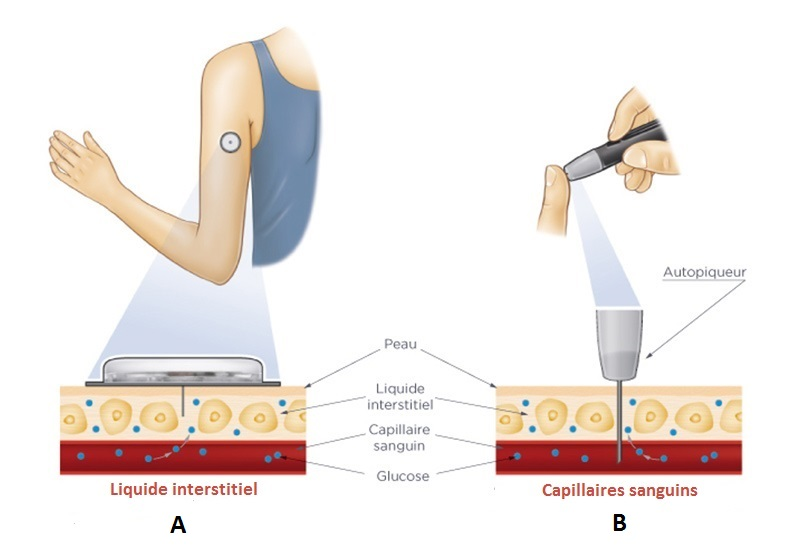
\includegraphics[scale=0.55]{images/glucometreVSfreestyle2.jpg}
        \caption{\label{fig:capillaireVSinterstitiel}Différents types de mesure de la glycémie.}
    \end{figure}
    
    
    La glycémie capillaire est la méthode la plus utilisée et nécessite l'utilisation d'un auto-piqueur (muni d'aiguilles à usage unique appelées lancettes), de bandelettes et d'un lecteur de glycémie. Un petit échantillon de sang est prélevé et déposé sur la bandelette puis analysé par le glucomètre.  (fig. \ref{fig:glycemieCapillaire})
    
    \begin{figure}[H]
        \centering
        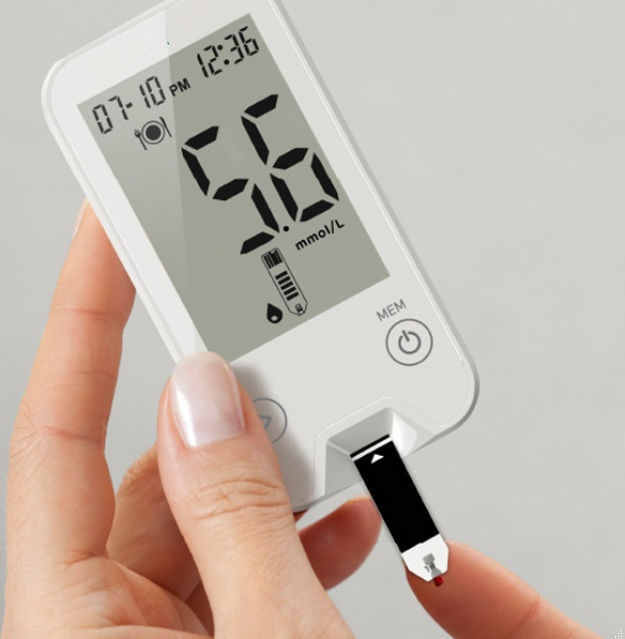
\includegraphics[scale=0.33]{images/glucometre.jpg}
        \caption{\label{fig:glycemieCapillaire}Système de mesure de la glycémie capillaire}
    \end{figure}

    
    Un système de mesure du glucose en continu (est composé d’un capteur posé à l'arrière du bras pendant 14 jours et d'un lecteur qui permet de scanner le capteur et de collecter les données.(fig. \ref{fig:systemeContinu}) 
    
    \begin{figure}[H]
        \centering
        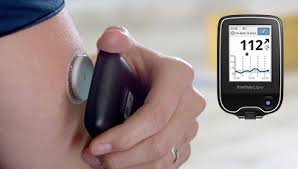
\includegraphics[scale=0.8]{images/glucometre2.jpg}
        \caption{\label{fig:systemeContinu}Système de mesure du glucose en continu}
    \end{figure}
    
    
    Les études ont montré que la quantité de glucose dans le milieu interstitiel reflétait le taux de glucose dans le sang mais avec un décalage de quelques minutes (au maximum 10 minutes) dans certaines situations:
    \begin{itemize}
        \item lorsque la glycémie est en train de baisser,
        \item lorsque la glycémie est en train d'augmenter\\
    \end{itemize}
    Ce décalage est principalement lié au temps de transfert du glucose entre le sang et le liquide interstitiel.\\
    
    
    Cependant après une course nous nous trouvons justement dans une de ces situations car la glycémie se modifie. Un système de mesure de la glycémie interstitielle  n'est donc pas adapté pour les athlètes qui souhaitent avoir leur glycémie immédiatement après un effort. Nous utiliserons donc un glucomètre classique pour l'étude.
    
    
    \vspace{10pt}
    
    
    \section{Lactatomètre}
    
    Un lactatomètre est un appareil permettant de mesurer la lactatémie (\autoref{subsection:lactatemie}). Elle est exprimée à l'écran en millimoles par litre de sang (mmol/L).\\
    
    Les lactomètres nécessitent l'utilisation d'un auto-piqueur pour le prélèvement du sang sur l'index ou le lobe de l'athlète ainsi que de bandelettes réactives, c'est à dire recouvertes d'une substance utilisée pour produire une réaction chimique. \\
    
    Un petit échantillon de sang est prélevé et déposé sur la bandelette puis analysé par le lactatomètre.

    Un des outil les plus répandus dans le monde du sport est le lecteur de lactate "Lactate Pro 2". \ref{fig:lactatePro2})
    
     \begin{figure}[H]
        \centering
        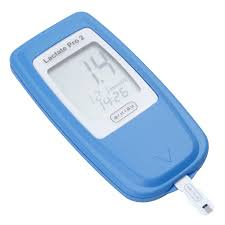
\includegraphics[scale=0.7]{images/lactatePro.jpg}
        \caption{\label{fig:lactatePro2}Lecteur de lactate "Lactate Pro 2"}
    \end{figure}
    
    Il mesure le taux de lactate en seulement 15 secondes par prélèvement d'une très faible quantité de sang (volume d‘échantillon d'uniquement 0,3 µl), sur l'index ou le lobe de l'athlète. De plus, toutes les données peuvent être transmises et archivées vers un PC de façon structurée grâce à l'interface USB intégrée. \\
    C'est cet outil que j'utiliserais dans la \autoref{section:priseLactate}.
    
    \vspace{10pt}
     
     
    \section{Montre connectée}
    
    La montre Forerunner 235 utilise un capteur optique qui mesure la fréquence cardiaque au poignet 24 heures sur 24 et 7 jours sur 7. Sa jauge de couleur identifie votre zone de fréquence cardiaque et vos battements par minute en temps réel.
    
     \begin{figure}[H]
        \centering
        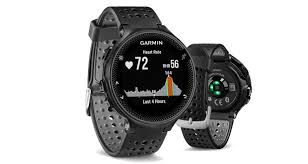
\includegraphics[scale=1]{images/garmin.jpg}
        \caption{\label{fig:garmin}Garmin Forerunner 235}
    \end{figure}

        
%%% Local Variables: 
%%% mode: latex
%%% TeX-master: "rapport"
%%% End: 

